\documentclass[a4paper]{article}

\usepackage{graphicx}
\usepackage{amsmath,amssymb}
\usepackage{minted}
\usepackage{multirow}
\usepackage{float}
\usepackage{todonotes}
\usepackage{forest}
\usepackage{xstring}
\usepackage{xcolor}
\usepackage[most]{tcolorbox}
\usepackage{xparse}
\usepackage{natbib}

\usetikzlibrary{graphs,graphdrawing}
\usegdlibrary{layered}

% for external graphviz
\input{/home/donkarlo/Dropbox/repo/nd_ai_project/src/nd_ai/knoweldge_representation/language/formal/computer/programming/tex/latex/code_clips/external_graphviz.tex}

% for tags
\input{/home/donkarlo/Dropbox/repo/nd_ai_project/src/nd_ai/knoweldge_representation/language/formal/computer/programming/tex/latex/parts/control_sequence/kind/semtag/semtag.tex}

% for links
\input{/home/donkarlo/Dropbox/repo/nd_ai_project/src/nd_ai/knoweldge_representation/language/formal/computer/programming/tex/latex/code_clips/seehere.tex}

\title{Open Building Footprints}
\date{}
\author{Mohammad Rahmani}

\begin{document}
    \maketitle
    
    
    \section{Open Building Footprints}
        Open building footprints describe the planimetric outlines of buildings as georeferenced polygons rather than as imagery.
        They provide stable building identifiers, approximate roof outlines, spatial relationships, and a direct geometry for selecting or clipping imagery.
        Footprints are useful for aligning multiple data sources and for calculating projected area when the polygon quality and coordinate reference system are known.
        They normally do not reveal roof material, slope, condition, or small rooftop structures, and their completeness and positional accuracy vary by location.
        Common sources include OpenStreetMap \seeherefooter{https://www.openstreetmap.org/} and Austria's open-data portal \seeherefooter{https://www.data.gv.at/}.
        
        \begin{figure}[H]
            \centering
            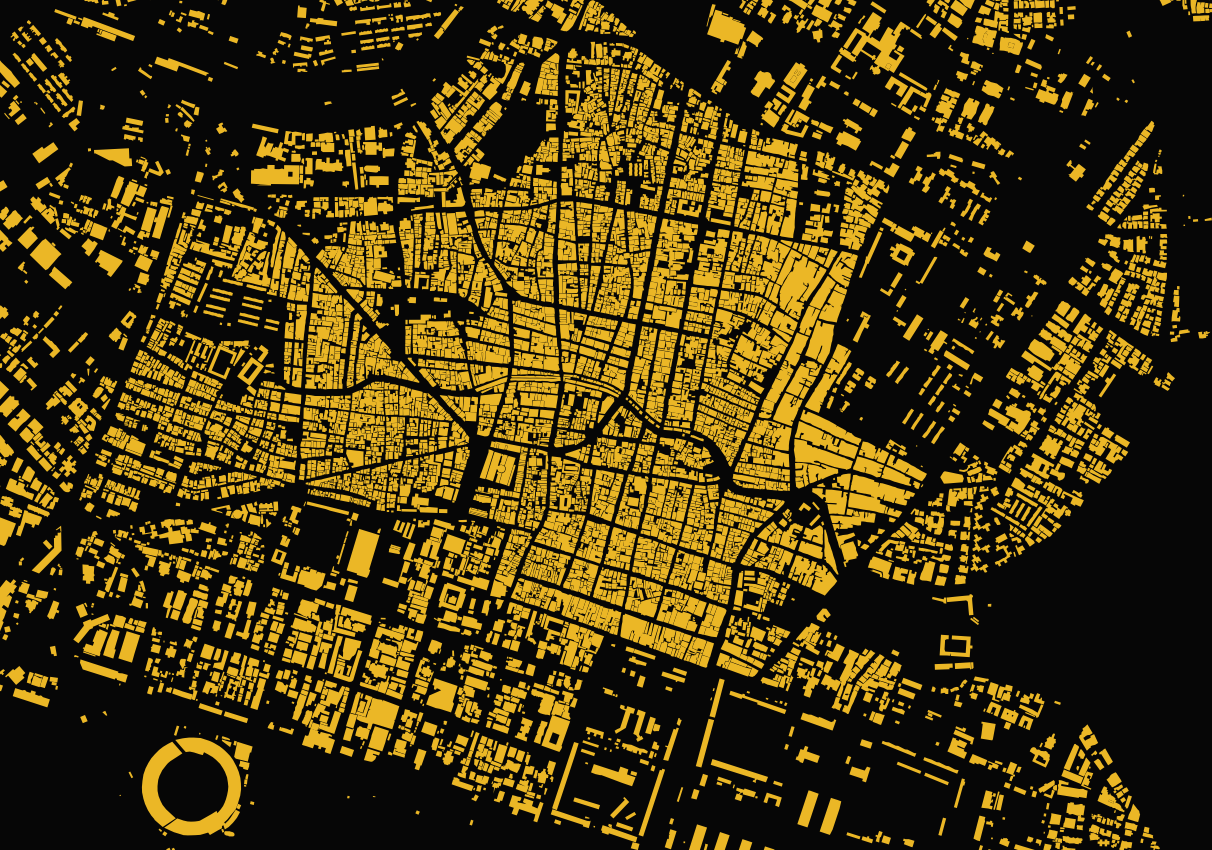
\includegraphics[width=0.88\textwidth]{images/open_building_footprints_example.png}
            \caption{Example rendering of a dense building-footprint dataset.}
        \end{figure}
        \noindent\small Image source and licence information: \seeherefooter{https://commons.wikimedia.org/w/index.php?oldid=836993207}.\normalsize
        
%        \bibliographystyle{plainnat}
%        \bibliography{/home/donkarlo/Dropbox/repo/nd_shared_research/bibliography/bibliography.bib}
\end{document}
